
\begin{appendices}

    % \renewcommand{\thesection}{П\arabic{secttion}}

    \section{ЯМР cпектры некоторых соединений}

    \begin{figure}[h!]
        \rotatebox{90}{
            \begin{minipage}{0.87\textheight}
                \includegraphics[width=\linewidth]{appendix/img/r19-1h.pdf}
                \caption{Спектр ЯМР \ce{^1H} соединения \cmpd{decafluoropyrazoline_substituted.piperidine}}
            \end{minipage}
        }
    \end{figure}

    \begin{figure}[h!]
        \rotatebox{90}{
            \begin{minipage}{0.9\textheight}
                \includegraphics[width=\linewidth]{appendix/img/r19-19f.pdf}
                \caption{Спектр ЯМР \ce{^19F} соединения \cmpd{decafluoropyrazoline_substituted.piperidine}}
            \end{minipage}
        }
    \end{figure}

    % % \begin{figure}[h!]
    % %     \rotatebox{90}{
    % %         \begin{minipage}{0.9\textheight}
    % %             \includegraphics[width=\linewidth]{appendix/img/r19-13c.pdf}
    % %             \caption{Спектр ЯМР \ce{^13C} соединения \cmpd{decafluoropyrazoline_substituted.piperidine}}
    % %         \end{minipage}
    % %     }
    % % \end{figure}

    \begin{figure}[h!]
        \rotatebox{90}{
            \begin{minipage}{0.87\textheight}
                \includegraphics[width=\linewidth]{appendix/img/ins.pdf}
                \caption{Спектр ЯМР \ce{^19F} реакционной смеси, полученной взаимодействием альдегида~\cmpd{decafluoropyrazoline_CHO} с 4-гидроксипиперидином
                    (мольное соотношение реагентов 2:3)}
            \end{minipage}
        }
    \end{figure}

    % % \begin{figure}[h!]
    % %     \rotatebox{90}{
    % %         \begin{minipage}{0.9\textheight}
    % %             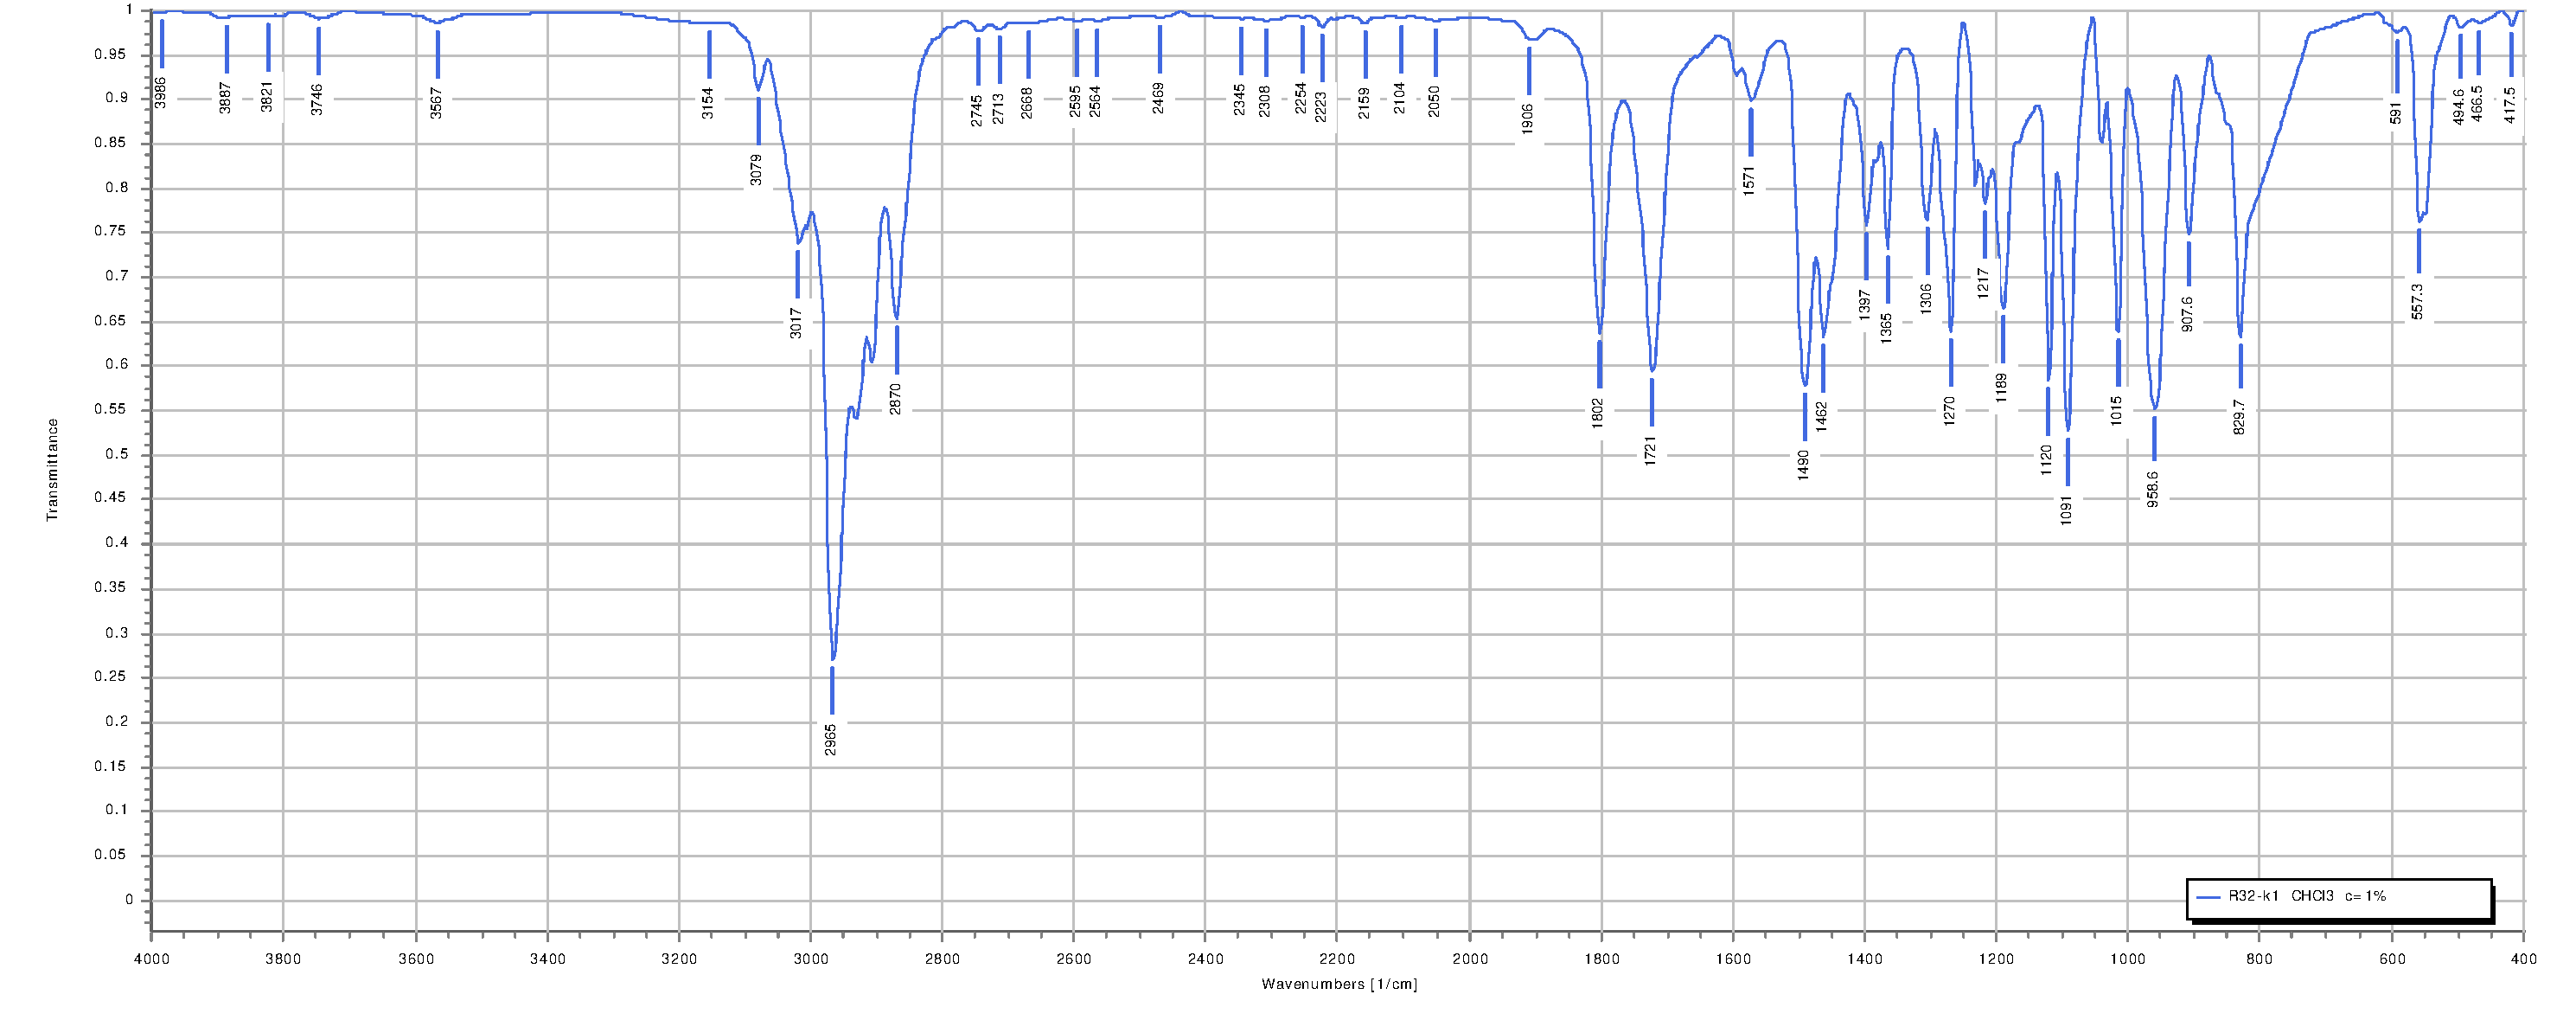
\includegraphics[width=\linewidth]{appendix/img/r32-k1.pdf}
    % %             \caption{ИК-спектр}
    % %         \end{minipage}
    % %     }
    % % \end{figure}

    \begin{figure}[h!]
        \rotatebox{90}{
            \begin{minipage}{0.9\textheight}
                \includegraphics[width=\linewidth]{appendix/img/r20-1h.pdf}
                \caption{Спектр ЯМР \ce{^1H} соединения \cmpd{decafluoropyrazoline_piperidine_benzoyl}}
            \end{minipage}
        }
    \end{figure}

    \begin{figure}[h!]
        \rotatebox{90}{
            \begin{minipage}{0.9\textheight}
                \includegraphics[width=\linewidth]{appendix/img/r20-19f.pdf}
                \caption{Спектр ЯМР \ce{^19F} соединения \cmpd{decafluoropyrazoline_piperidine_benzoyl}}
            \end{minipage}
        }
    \end{figure}

\end{appendices}
